\documentclass[12pt]{article}
\usepackage[utf8]{inputenc}
\setlength{\parindent}{0em}
\usepackage{amsmath}
\usepackage{amsfonts}
\usepackage{amssymb}
\usepackage[natbib=true, style=apa]{biblatex}
\usepackage{hyperref, url}
\usepackage{graphicx, float, subcaption}
\addbibresource{report.bib}
\usepackage{fullpage}
\usepackage{pdfpages}
\usepackage{listings}
\usepackage{color}
\usepackage{enumitem}
\definecolor{dkgreen}{rgb}{0,0.6,0}
\definecolor{gray}{rgb}{0.5,0.5,0.5}
\definecolor{mauve}{rgb}{0.58,0,0.82}

\lstset{frame=tb,
  language=C,
  aboveskip=3mm,
  belowskip=3mm,
  showstringspaces=false,
  columns=flexible,
  basicstyle={\small\ttfamily},
  numbers=none,
  numberstyle=\tiny\color{gray},
  keywordstyle=\color{blue},
  commentstyle=\color{dkgreen},
  stringstyle=\color{mauve},
  breaklines=true,
  breakatwhitespace=true,
  tabsize=3
}

\title{Augmented Reality Guidance for CT Spinal Injections}
\author{Sarah Gauthier, Chayce Ross, Henrique Saito, Sumin Olivia Kim}
\date{12th April 2024}
\begin{document}
\maketitle
\begin{figure}[H]
    \centering
    
\includegraphics[width=0.7\textwidth]{"./figs/quest_controller.jpg"}
    \label{fig:controller_header}
\end{figure}
\begin{center}
\subsection*{Project Sponsor}
Philip Edgcumbe - UBC Radiology\\
\subsection*{Project 2405}
ENPH 459 \\
Engineering Physics Project Lab \\
University of British Columbia  \\
\end{center}
\pagebreak



\pagebreak
\tableofcontents
\pagebreak
\listoffigures
\pagebreak
\section{Introduction - Olivia}
\subsection{Background}

Spinal injections are a common medical procedure involving the injection of medication near specific nerves in the spinal area to relieve pain. These procedures are performed by neuroradiologists who use CT scans of the patient's spine to guide the injection needle to the desired location. To ensure precise needle placement, physicians must take multiple CT scans of the patient's spine at different angles to confirm that the needle is correctly inserted. This is a long process that exposes patients and physicians to harmful radiation. Additionally, due to the trial-and-error nature of this procedure, it may require multiple needle insertion attempts, each involving a series of CT scans.\\

To reduce the number of CT scans and needle insertion attempts required, we propose an Augmented Reality (AR) tool, using the Meta Quest 3 headset, to guide these spinal injection procedures.
 
\subsection{Team Introduction - Sponsors and Students}

This project is sponsored by Dr. Philip Edgcumbe, a resident physician, entrepreneur, biomedical engineer and clinician-scientist (MD, PhD) working in Diagnostic Radiology at the University of British Columbia (UBC). Dr. Edgcumbe also holds a BASc in Engineering Physics from UBC, obtained in 2011. He has invented, patented and licensed an augmented reality navigational aid for surgery and co-founded two biomedical start-up companies. Given his extensive background in both medicine and engineering, Dr. Philip Edgcumbe was able to provide excellent guidance and support throughout this project.\\

In addition to Dr. Edgcumbe, Dr. Will Guest (MD, PhD, BSc), a neuroradiologist at the Vancouver General Hospital (VGH), provided supervisory support.\\

The student team is comprised of four 4th-Year Engineering Physics students at UBC: Sarah Gauthier, Chayce Ross, Henrique Saito and Sumin Olivia Kim. 

\subsection{Discussion with Stakeholders}
Prior to developing this AR solution, the team held discussions with stakeholders to accurately scope project needs. Dr. Will Guest, a staff physician at the Vancouver General Hospital was a key stakeholder in this project, with in-depth experience with spinal injections and radiology.\\

During an interview conducted at the Vancouver General Hospital, Dr. Guest described in detail the steps involved in a spinal injection (which we outline in \ref{spine-procedure:Overview of Spinal Injection Procedure}). He also explained the limitations of the current procedure. He mentioned that the procedure can be uncomfortable to perform for physicians as the patient needs to be lying inside the CT scanning unit at all times. If a patient has a large torso, they may take up most of this area, making it difficult to insert the needle at the right angle.\\ 

Dr. Guest expressed that having the patient's bony structures projected onto their body during this procedure would be a great asset to neuroradiologists as they would be able to insert the needle using with less iterative CT scans, and perform the injections more quickly.

This interview allowed the engineering team to assess the key project objectives.\\

\href{https://www.youtube.com/watch?v=NSqduAn1Zb4}{This video shows the steps of a CT-guided spinal procedure, by Dr. Will Guest.}

\subsection{Overview of Spinal Injection Procedure} 
\label{spine-procedure:Overview of Spinal Injection Procedure}

Spinal injection procedures are used primarily to relieve pain by delivering medication directly to the spinal nerves' vicinity, and are often employed in cases of chronic back pain, sciatica, herniated discs, and spinal stenosis, among other conditions.\\
\\
The procedure involves patient preparation, precise needle insertion guided by imaging techniques (such as fluoroscopy or CT scans), and medication delivery directly to the pain site. \\
\begin{enumerate}
    \item \textbf{Patient Preparation:} Before the procedure, patients receive a comprehensive evaluation where the risks and benefits are explained. This phase also involves monitoring vital signs and positioning the patient.
    
    \item \textbf{Initial CT Scan:} A CT scan of the patient's spinal region is done to accurately locate the optimal needle insertion trajectory. This imaging m
    odality provides real-time visuals of the spine, enabling precise needle guidance to the affected area.
    
    \item \textbf{Sterilization and Anesthesia:} The skin over the targeted site is meticulously cleaned and sterilized to minimize infection risks. A local anaesthetic is then administered to numb the area, reducing discomfort during needle insertion.
    
    \item \textbf{Initial Needle Insertion:} With the patient still inside the CT scanning unit, a needle is inserted through the skin, about 1cm deep, and meticulously directed toward the area adjacent to the spinal nerves.

    \item \textbf{Verification CT Scan:} The physician takes another CT scan of the patient with the needle inserted. The needle's position is checked. If the needle is in the right position, the physician moves on to the next step. Otherwise, they remove the needle and return to the initial needle insertion step.

    \item \textbf{Deeper Needle Insertion:} The physician pushes the needle in slightly deeper. The needle's placement is continuously adjusted based on imaging feedback until the optimal position is confirmed. Subsequently, the medication—commonly a steroid or anesthetic—is injected to diminish inflammation and mitigate pain.

    \item \textbf{Procedure Conclusion:} Upon successful medication delivery, the needle is carefully withdrawn, and the injection site is cleaned and bandaged. Post-injection, patients are observed for a brief period to monitor for adverse reactions.
\end{enumerate}

\subsection{Previous Work - Chayce}
This work is inspired by a previous paper (\cite{HoloInjections}) that tested and compared different assistance and guidance techniques for needle insertion procedures using the \href{https://www.microsoft.com/en-ca/hololens}{Microsoft Hololens}, an AR headset. In this paper, the researchers used the HoloLens to project a needle trajectory above a foam block. The user would try to match the trajectory and insert a needle into the foam. The goals of the paper were to:
\begin{enumerate}
    \item Find out if AR headsets are a viable form of guidance for surgical settings.
    \item Compare the effectiveness of different visualization methods for guidance, including the intersection of two planes, a line, and a cone (Figure~\ref{fig:cones}). 
\end{enumerate}
\begin{figure}[H]
    \centering
    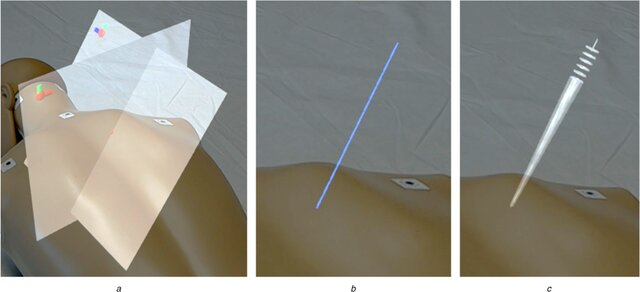
\includegraphics[width=0.9\textwidth]{figs/cones.jpg}
    \caption{Different guidance methods for injections compared in the HoloInjections paper (\cite{HoloInjections}). \textbf{(a)} Intersection of planes, \textbf{(b)} line, \textbf{(c)} cone.}
    \label{fig:cones}
\end{figure}
\paragraph{Methodology/Evaluation} To test these different guidance cues, the authors of this paper chose a trajectory angle at random and asked the user to follow it. After the user inserted the needle completely into the block, they measured the difference between the expected endpoint and the actual endpoint of the needle. The authors evaluated each injection by two criteria:
\begin{enumerate}
    \item \textbf{In-Plane Accuracy:} Remembering that each injection is conducted in the \textbf{transverse plane} of the patient, this measures the difference in angle between the expected and actual angles in the transverse plane.
    \item \textbf{Out-of-Plane Accuracy:} This measures the smallest angle between the transverse plane of the patient and the angle of the needle.
\end{enumerate}

After testing, the authors found that the \textbf{cone} was the most accurate and intuitive method for guidance. They also concluded that the HoloLens was not accurate enough to use for AR guidance and some improvements would need to be made to the tracking sensors in the headset. Moreover, the Hololens uses a ``projection" technique to create AR environments. To do this, it projects items onto a glass screen in front of the user's eyes. This allows for clear vision into the real world but does not allow the 3D objects to be ``embedded'' into the user's environment. Rather, to the user, everything appears behind the projections. This makes it hard to sense depth as the user cannot tell when they have passed the intended point of insertion between the projection and the real world.\\

Given these important conclusions and our own research, we have chosen to pursue the Meta Quest 3 headset given that it has greater depth perception to allow the user to interact with the projections more naturally.

\subsection{Problem Statement}
Spinal injection procedures currently rely on multiple CT scans to guide needle placement. This traditional method exposes patients and healthcare providers to significant radiation and often requires numerous needle adjustments, making the process time-consuming and prone to errors. There is a critical need for a solution that enhances precision, reduces radiation exposure, and streamlines the procedure to improve patient outcomes and safety. 

\subsection{Proposed Solution}
\label{sec:ProposedSolution}
Our proposed solution leverages augmented reality (AR) technology to enhance the accuracy, safety, and speed of spinal injection procedures. By using an AR headset, we can provide the user with a real-time, three-dimensional visual guidance system, embedded directly into the operating environment.\\
\\
The core of our solution involves overlaying a virtual image of the patient’s anatomical structures onto their actual body as viewed through the AR headset. This ``X-ray vision" feature allows the physician to see the target area for the needle insertion without the need for repeated CT scans, reducing radiation exposure for both patient and healthcare providers.\\
\\
Additionally, our AR system projects the optimal needle trajectory into 3D space. This pathway guides the physician in real-time, suggesting the best angle and depth for needle insertion.

\subsection{Project Objectives}
The project aims to develop a user-friendly augmented reality solution to expedite spinal injection procedures. The AR solution should achieve the following, in order of importance:
\begin{enumerate}
    \item Reduce the total operative time of the spinal injection procedure
    \item Reduce the average number of CT scans performed on the patient, thereby reducing their exposure to radiation
    \item Reduce the average number of needle insertion attempts required per procedure
    \item Reduce patient discomfort during the procedure
\end{enumerate}

\section{Discussion}
\subsection{Theory}
\subsubsection{Computerized Tomography (CT) Scans - Sarah}
To perform spinal injections, physicians must find the ideal injection trajectory; one that avoids bony structures while targeting the desired nerves. This is done using computerized tomography (CT) scans of the patient's spine. A CT scan is a diagnostic tool that uses X-ray beams to produce images of a patient's anatomical structures (John Hopkins \cite{HopkinsMed}). X-rays are beams of high-energy electromagnetic radiation that are ``absorbed in different amounts depending on the density of the material they pass through" (Mayo \cite{MayoClinic}). The denser the material is, the lighter it will appear in the X-ray or CT scan image. Thus, bones and metals are easily identifiable on these types of scans since they appear white.\\ 

We can therefore leverage the fact that metal is easily identifiable in CT scans to link the structures of the CT scans to the patient's body in the real world. We will explain this process in greater depth in Section \ref{reg:Registration}.\\

\begin{figure}[H]
    \centering
    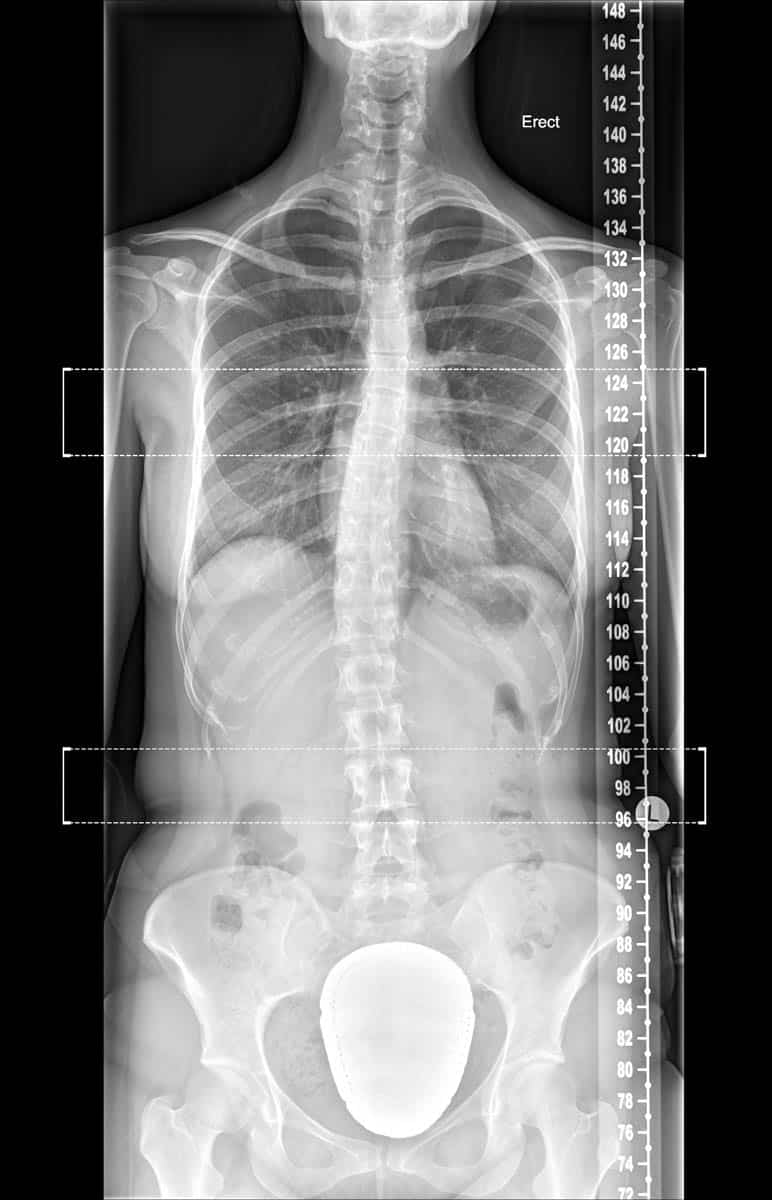
\includegraphics[width=0.3\textwidth]{figs/x_ray.jpeg}
    \caption{X-Ray image of a spine}
    \label{fig:x_ray}
\end{figure}

To produce CT scans, a patient is placed inside a CT scanning unit, which is a large cylindrical tube. They are then slowly pushed through this tube while an X-ray beam is aimed at the patient and quickly rotated around their body (Figure \ref{fig:ct_unit}).\\

\begin{figure}[H]
    \centering
    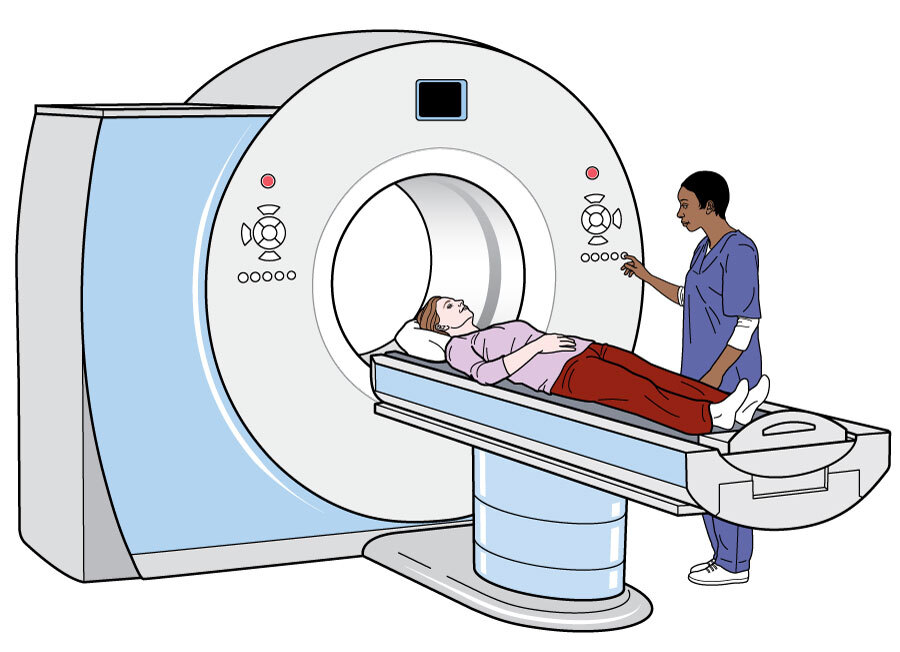
\includegraphics[width=0.5\textwidth]{figs/ct_scanner.png}
    \caption{Animation of a patient inside a CT scanning unit}
    \label{fig:ct_unit}
\end{figure}

This produces a series of cross-sectional images, or "slices" of the patient's body (Figure \ref{fig:ct_stack}). These images can then be stacked and rendered to form a three-dimensional object of the patient's anatomy.

\begin{figure}[H]
    \centering
    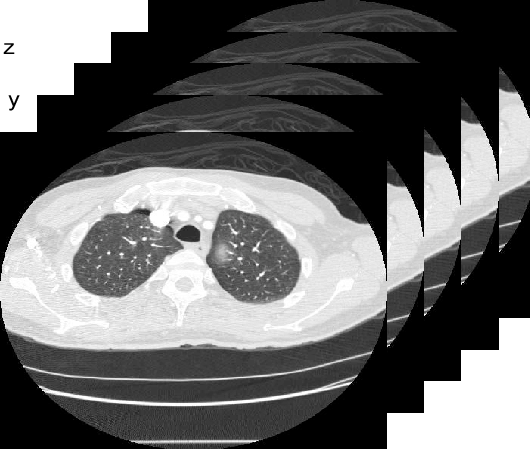
\includegraphics[width=0.4\textwidth]{figs/ct-stack.png}
    \caption{A stack of 2D cross-sectional CT scans}
    \label{fig:ct_stack}
\end{figure}

\subsubsection{Augmented Reality - Henrique}
Augmented Reality (AR) is a type of immersive technology that allows the user to see both the virtual rendered world and the real physical world around them. It provides the user with ``visual elements, sound and other sensory information [...] through a device like a smartphone, glasses or a headset" (\cite{ar}). We can leverage this technology to give doctors all the necessary information they need for the procedure while simultaneously allowing them to keep eyes on the operation. In other words, this allows us to give guidance without interfering with the doctor's focus or workflow.\\ 

There are various head-mounted displays (HMD) (i.e. headsets) that support augmented reality, with varying quality. Important factors to consider include spatial mapping precision and pass-through resolution.

\subsubsection{Unity}
In this project, Unity serves as the core development environment for creating AR applications designed to run on headsets.\\

Unity’s platform allows developers to utilize features such as controller tracking, spatial anchoring, and interactive visual overlays to create immersive AR experiences that are stable and responsive. It also allows developers to download software development kits (SDKs) for different headset types to the platform, which greatly helps the development process. After development, the Unity application can be loaded onto the headset and tested.

\subsubsection{Registration}
\label{reg:Registration}
In order to map the coordinate system for the fiducials in the CT scans \(x_c\)  (``CT fiducials") to the fiducials in our game world \(x_p\) (``physical fiducials"). Where each fiducial $x_{ci}$ is transformed by $\underbar{x}_i = \underbar{t} + s \cdot \textbf{R} \underbar{x}_{ci}$. Where $\underbar{t}$ is a translation vector, $s$ is a scalar scaling factor and $\textbf{R}$ is a rotation matrix. This process of mapping the two virtual coordinate systems together is called ``Registration''. 

\subsection{Design \& Approach}

\subsubsection{Proposed User Experience and Workflow}
To achieve our project objectives, we propose a system that allows neuroradiologists to visualize both the patient's internal anatomy and the optimal needle insertion trajectory during spinal injections.\\

When utilizing our developed AR solution, the physician would perform spinal injections following these steps (illustrated in Figure \ref{fig:work-flow}):
\begin{enumerate}
    \item The physician places metal fiducial markers on the patient's back near the injection site.
    \item The physician performs a CT scan of the patient's torso with the fiducial markers present.
    \item The physician puts on the Quest 3 headset. The CT scan data is loaded into the headset and is projected in front of the user.
    \item The physician scrolls through all the CT slices using a scroll bar below the images. When they see a white dot at the top of the CT scan, they click on it to register it as a CT fiducial marker. When all the fiducials are identified, the physician selects a desired CT slice to annotate with the optimal needle trajectory.
    \item The physician opens the CT scan annotation applet in the headset. They select two points on the CT slice using the controller. A red line joining these two points is created on the CT slice.
    \item The stack of 2D CT slices is \textbf{rendered into a 3D object} (\ref{mesh:3D Meshing with Marching Cubes}) representing the patient's spine. The annotation of the needle trajectory is rendered on the object.
    \item The physician takes the controller with the pointer tip attachment and opens the fiducial registration applet in the headset. They tap each fiducial marker one at a time to \textbf{register their coordinates as spatial anchors} (\ref{spa:Spatial Anchors}).
    \item The fiducial markers on the 3D spinal object are \textbf{mapped to the fiducial markers on the patient's torso using a coordinate transformation} (\ref{coord:Coordinate Transform using Horn's Method}). The physician sees the needle trajectory and the patient's internal anatomy projected on their body.
    \item The physician attaches the needle to one of the controllers using a custom attachment piece. The controller allows the \textbf{needle's location to be continuously tracked} (\ref{cont:Controller Tracking and Attachments}). Wearing the headset, the physician follows the projected trajectory with the needle attached to the controller.
    \item The physician receives feedback on their alignment with the optimal trajectory.
\end{enumerate}

The above components that are \textbf{bolded} have been developed by our team. In the following sections, we provide an overview of the critical design decisions made when developing these components.

\begin{figure}[H]
    \centering
    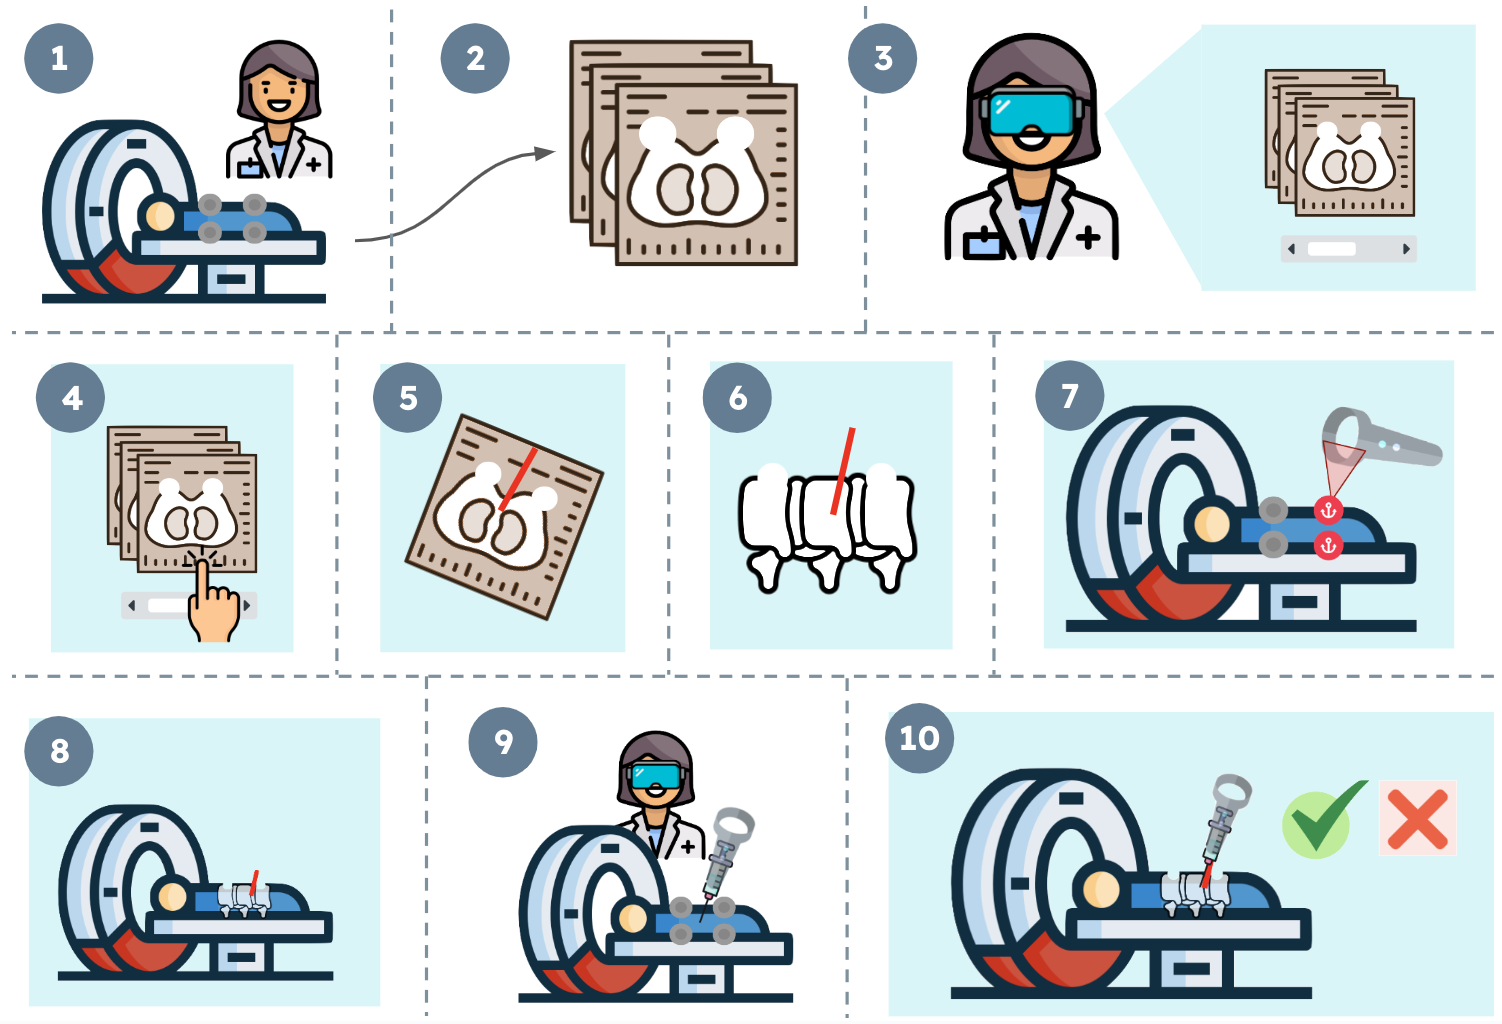
\includegraphics[width=0.9\textwidth]{figs/newer-workflow.png}
    \caption{Proposed user experience using AR}
    \label{fig:work-flow}
\end{figure}


\subsubsection{Controller Tracking and Attachments}
\label{cont:Controller Tracking and Attachments}
For both tracking the needle and registering fiducials, we must have a method of knowing the exact coordinates of real-world tools in the headset's frame of reference. We can do this by using the two controllers that come with the Quest 3 headset. These controllers are automatically being tracked by the headset using IR beacons, and so we can attach the needle or a pointer to the controller and by proxy know its coordinates.\newline

In software, each controller has a set of cartesian coordinates with respect to the world. These coordinates represent the location of a specific point on the controller. We can call this point the ``tracking anchor". Unfortunately, the tracking anchor of the Quest 3 controller is at a seemingly arbitrary location on the face of the controller (Figure \ref{fig:controller_anchor}).

\begin{figure}[H]
    \centering
    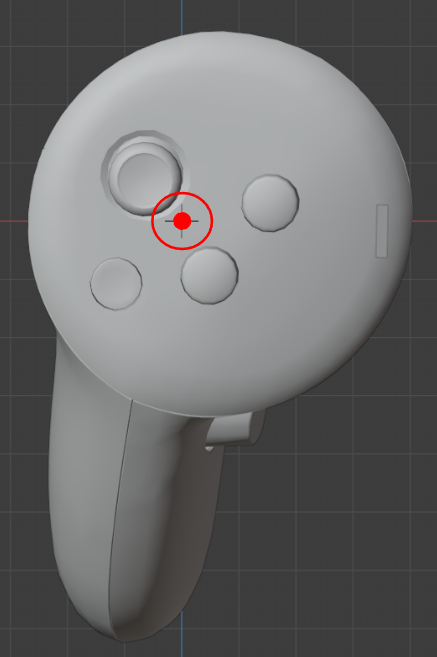
\includegraphics[width=0.3\textwidth]{figs/controller_anchor.png}
    \caption{Quest 3 controller tracking anchor point}
    \label{fig:controller_anchor}
\end{figure}

Thus, the core technical problem is to find the offset between the controller's tracking anchor and the desired point that needs to be tracked (needle or pointer end). In other words, we must find the black vector illustrated in Figure \ref{fig:controller_pointer_diagram}, which shows an example pointer attachment.

\begin{figure}[H]
    \centering
    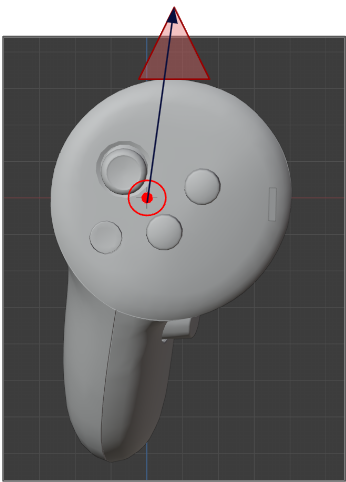
\includegraphics[width=0.3\textwidth]{figs/controller_anchor_pointer.png}
    \caption{Unknown vector between anchor point and pointer tip}
    \label{fig:controller_pointer_diagram}
\end{figure}

Our initial plan was to lock down the end of the pointer in one spot with a purpose-built rig (as an example, see Figure \ref{fig:controller_calibration_rig}). We then rotate the controller around and record the Cartesian coordinates and rotation of the controller at three different spots. We can convert the rotation to a directional vector, which combines with the Cartesian coordinates to form a line equation. By finding the intersection of these lines, we can then find the desired point and thus the unknown vector. 

\begin{figure}[H]
    \centering
    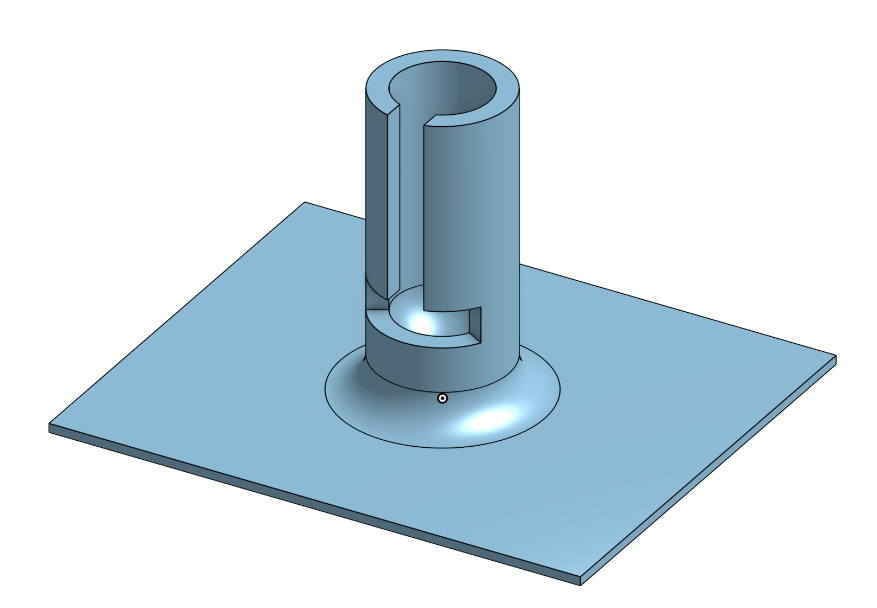
\includegraphics[width=0.5\textwidth]{figs/calibration_rig.png}
    \caption{Example calibration rig to keep end point static}
    \label{fig:controller_calibration_rig}
\end{figure}


If the three lines were guaranteed to intersect, finding the intersection would be trivial. Unfortunately, the lines will note exactly intersect, so a least-squares approximation has to be used to find the point which minimizes the distance to each of the lines. A system diagram can be found in figures \ref{fig:old_calibration_diagram} and \ref{fig:old_calibration_diagram2}.

\begin{figure}[H]
    \centering
    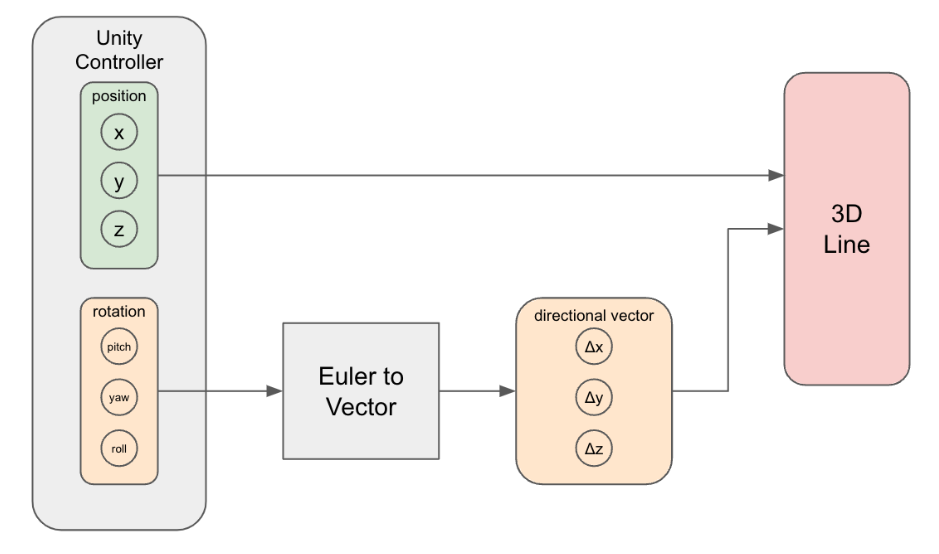
\includegraphics[width=0.7\textwidth]{figs/old_calibration_diagram_1.png}
    \caption{System diagram for each recorded controller location}
    \label{fig:old_calibration_diagram}
\end{figure}

\begin{figure}[H]
    \centering
    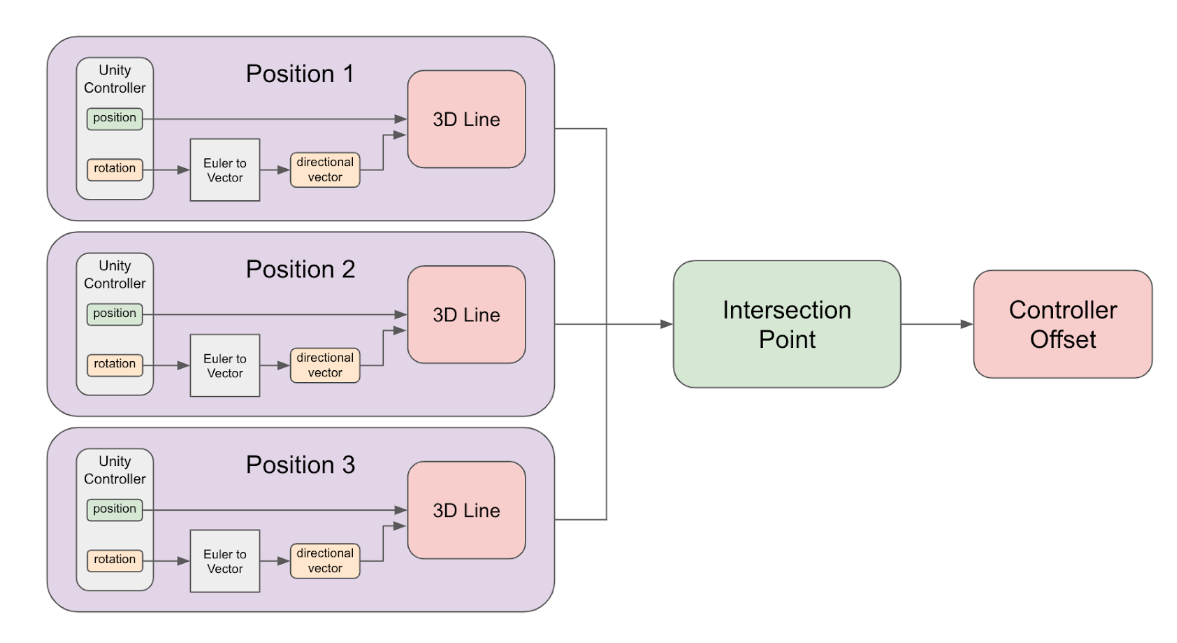
\includegraphics[width=0.9\textwidth]{figs/old_calibration_diagram_2.png}
    \caption{Finding intersection between lines}
    \label{fig:old_calibration_diagram2}
\end{figure}

Unfortunately, this approach has a fatal flaw. The aforementioned procedure has an inherent assumption that the controller attachment is pointing in the same direction as the controller's internal direction. If the attachment was pointing to the left of the controller's face, for example, the lines would never all intersect and the least squares approximation would not return the correct point (Figure \ref{fig:old_calibration_diagram3}).

\begin{figure}[H]
    \centering
    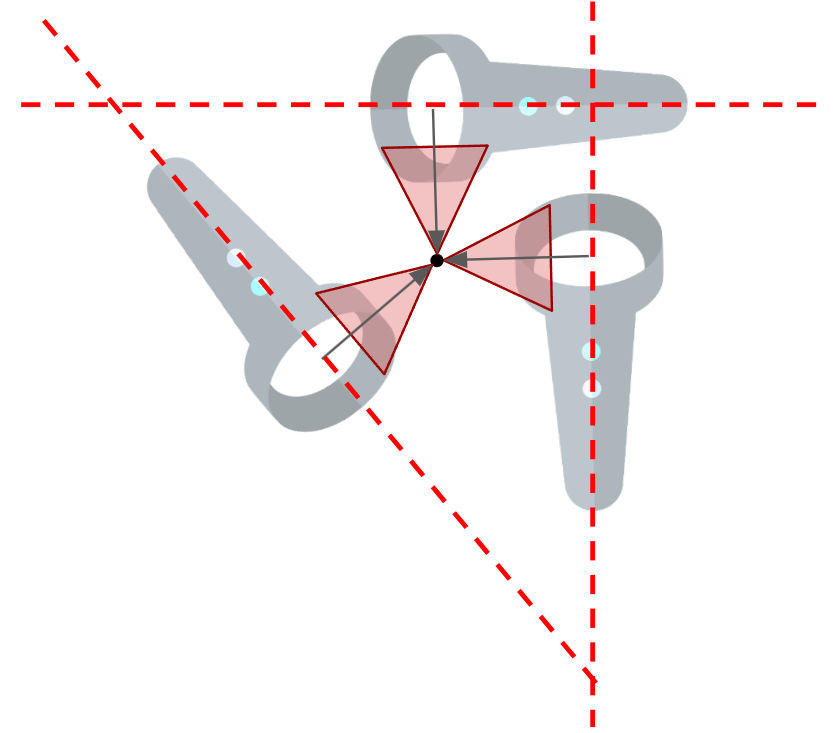
\includegraphics[width=0.5\textwidth]{figs/old_calibration_diagram_3.png}
    \caption{If the pointer attachment pointed left, the lines would never intersect}
    \label{fig:old_calibration_diagram3}
\end{figure}

Instead, we can do a similar procedure, where we still keep the pointer end static and then rotate the controller about the pointer end. We can then record four different sets of coordinates as the controller moves around. Note that because the length of the pointer is constant, and the location of the endpoint is also constant, the four coordinates we have collected will define the surface of a sphere. If the coordinates were all exactly on the surface of the sphere, it is then trivial to find the centre of the sphere, and thus the coordinates of the pointer end, but this is not the case. Instead, we have to optimize the 3 parameters, which correspond with the Cartesian coordinates of the pointer end, such that the variance in distance between each recorded set of coordinates and the 3 parameters, is as low as possible. Thus we have our cost function:

$$\text{Cost} = \frac{1}{4}\sum^{4}_{i=1}(r_i - \bar{r})^2$$

where $r_i$ represents the distance between the $i$th recorded coordinates and the proposed centre and $\bar{r}$ represents the mean distance between all of the recorded coordinates and the proposed centre.\\

Software aside there exist further considerations about the controller attachments. Taking off and putting back on the attachment may end up with slightly different positioning, so ideally we keep the attachments permanently on the controllers. Luckily for us, we have two controllers and two separate attachments. Another further consideration is the attachment mechanism to the actual medical needle. We have decided to delay designing for the needle until the underlying engineering work is done.\\

Lastly, there is one final consideration in the medical context. In an operation, the common rule of thumb is that everything below the doctor's neck must be sterilized. This means while we do not have to worry about the sterilization of the headset, we must sterilize the controllers. The easiest solution is to place the controllers inside sterilized plastic bags, which are custom-made for sterilizing non-medical tools. There is a concern that the plastic bag will interfere with the IR tracking beacons on the controller, but like the needle attachment design, we will delay this decision.

\subsubsection{Spatial Anchors}
\label{spa:Spatial Anchors}
To translate the real world into the AR space, physical objects on the patient's body (metal fiducial markers) are registered as spatial anchors.\\

Spatial anchors are digital markers that allow AR environments to accurately anchor virtual objects to specific locations in the real world. This ensures that virtual content appears stable and remains in the correct real-world position, even as the user moves and interacts with the environment.\\
\\
\textbf{SDKs}\\
\\To build spatial anchors within Unity for the Meta Oculus Quest 3 headset, several SDKs and integration packages were used. Specifically, the Meta Oculus Integration package (deprecated) as well as the Meta All-In-One SDK provided extensive support for the creation, customization and data extraction for spatial anchors. Using these two packages, two sets of preliminary spatial anchor prototypes were created.\\
\begin{figure}[H]
    \centering
    \begin{minipage}{0.49\textwidth}
        \centering
        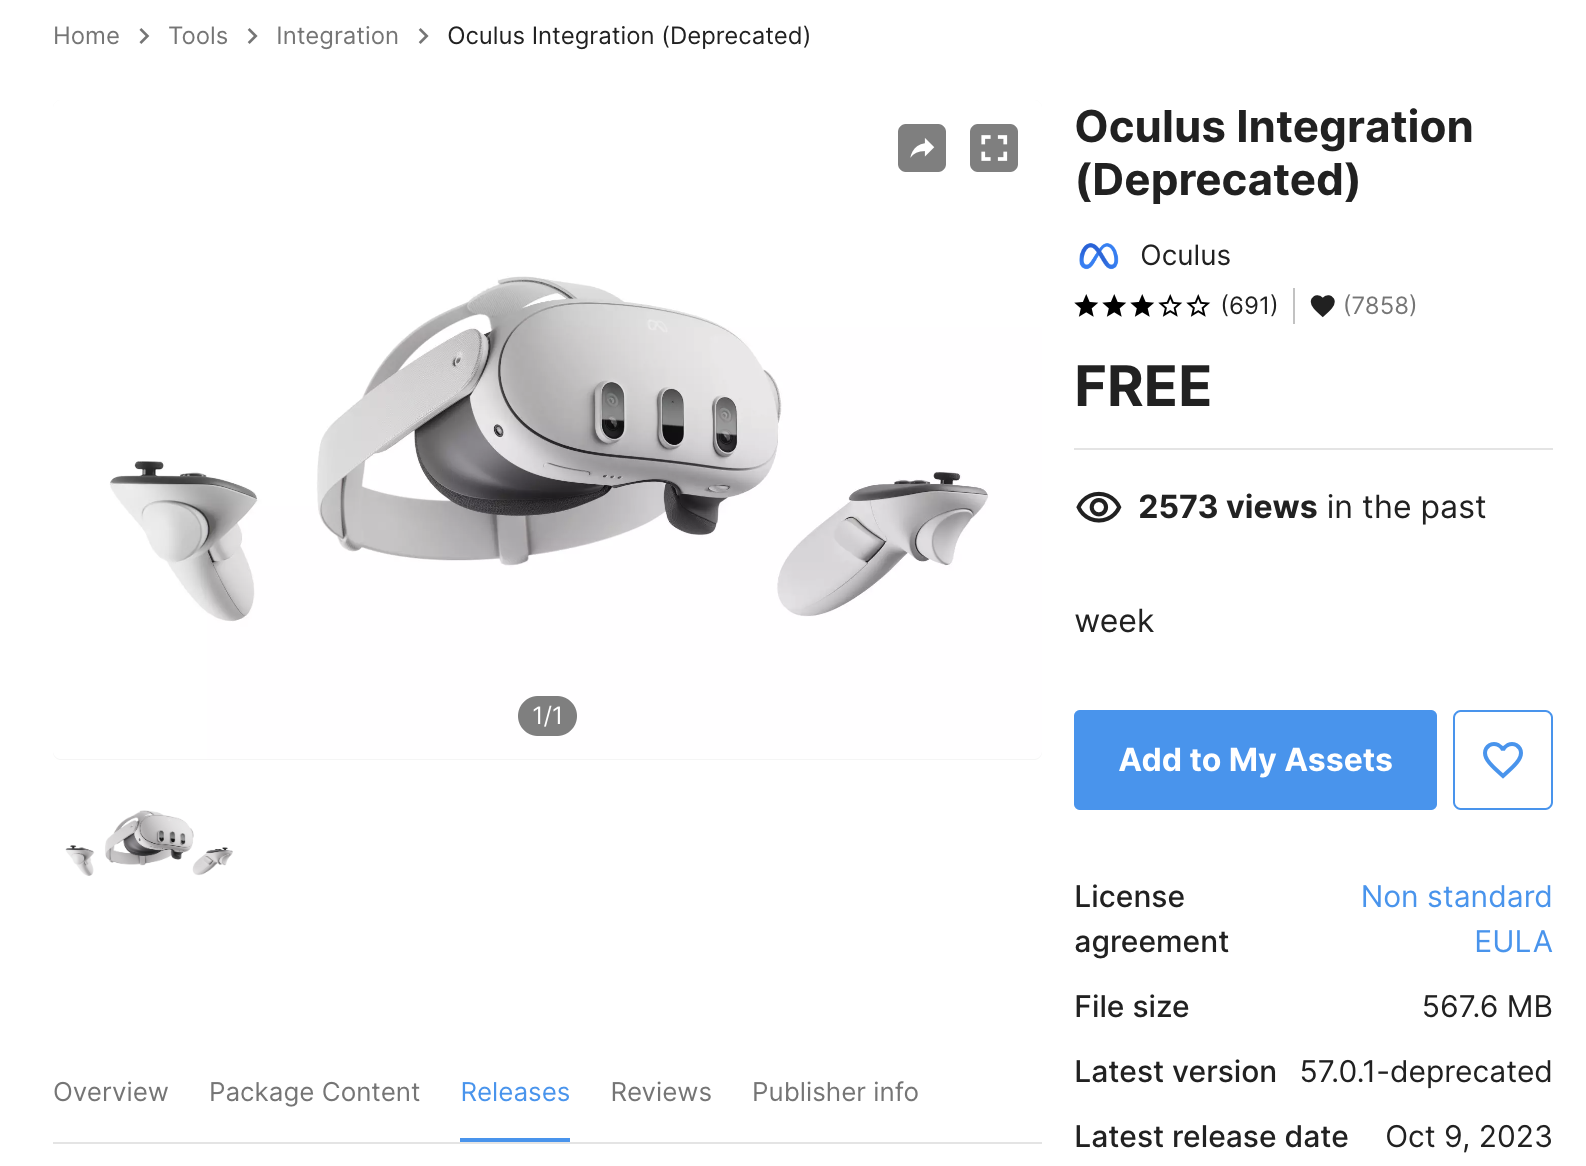
\includegraphics[width=\textwidth]{figs/oculus-int.png}
        \caption{Meta Oculus Integration package}
        \label{fig:oculus-int}
    \end{minipage}\hfill
    \begin{minipage}{0.49\textwidth}
        \centering
        
\includegraphics[width=\textwidth]{figs/meta-all.png}
        \caption{Meta All-In-One SDK}
        \label{fig:meta-all}
    \end{minipage}
\end{figure}
\\
\textbf{Prototype 1:  Oculus Integration (deprecated)}\\
\\
The Oculus Integration package (release: 07/2017) provides several Oculus Unity SDK integrations as a single Unity asset, as well as an extensive range of existing examples, tutorials and documentation. This abundance of resources made it a straightforward process to develop the first prototype.\\
\\
This prototype, derived from Meta’s Unity StarterSamples, incorporates XR features such as controller tracking, 3D location markers, anchor placement, and various tools for interacting with anchors—specifically, selecting, moving, and deleting them.\\
\\
This model features a user menu with two options: "Create Anchor" and "Select Anchor." In the "Create Anchor" mode, the user sees the controller, which displays location tracking lines to guide placement of the anchor in 3D space. Users can then place the anchor, represented by a small anchor icon—a custom prefab specified within Unity—at the chosen location. Once placed, the anchor remains fixed in that position, allowing users to observe that it does not move as they interact with and move around their environment. In the "Select Anchor" mode, users can select previously placed anchors, move them, or delete them as needed.\\
\\
Despite these capabilities, the prototype primarily depended on APIs and packages that Meta has recently deprecated. This raised concerns about the prototype’s scalability and long-term maintainability, which are critical considerations given that the project is expected to span several years. Since precise and reliable spatial anchoring is essential for accurately displaying AR overlays, the continued use of this deprecated integration poses significant risks to the project’s future effectiveness and support. Therefore, evaluating alternatives or updates becomes a priority to ensure the longevity and robustness of the system in handling AR elements within a medical setting.

\begin{figure}[H]
    \centering
    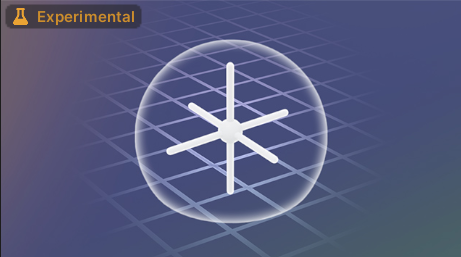
\includegraphics[width=0.3\textwidth]{figs/spatial_anc.png}
    \caption{Spatial anchors in AR}
    \label{fig:spatial_anc}
\end{figure}

\subsubsection{3D Meshing with Marching Cubes}
\label{mesh:3D Meshing with Marching Cubes}
An important part of our proposed user experience is the use of a 3D model in our game engine for the user to see the bone structure in real time. There are many online applications that can take CT scans and turn them into surface meshes. However, we cannot use them as we would like all data to stay on the device. Moreover, we want to ensure that we can render our surfaces as soon as the CT scan is conducted (i.e. at runtime). As a result, we have implemented an algorithm for meshing called ``Marching Cubes'' (\cite{MarchingCubes}), that runs in parallel on the Graphics Processing Unit (GPU) on the headset. Below, we will walk through our implementation, describe the algorithm and define some necessary to understand terms. 
\paragraph{3D/Surface Meshes:} Unity renders 3D objects using a {\bf polygon mesh} (Figure~\ref{fig:3d_reps}(iii)). A polygon mesh is a list of triangles situated in 3D space that reflect light (based on the texture of their assigned material). A smooth 3D object is created by placing triangles along the surface of the object to form a 3D shape.
\paragraph{Voxels and Point Clouds:} Recall that the CT scan returns a stack of CT images. These can be layered on top of each other into a 3-dimensional tensor, where each element is a number between 0 and 1 (where the 1s are the brightest values representing the most dense structures in the anatomy). This 3D tensor can be envisioned in two ways:
\begin{enumerate}
    \item Voxels: each element in the tensor represents a cube in 3D space.
    \item Point Cloud: each element in the tensor represents the corner of a cube in 3D space.
\end{enumerate}
These are illustrated in Figure~\ref{fig:3d_reps}.
\begin{figure}[H]
    \centering
    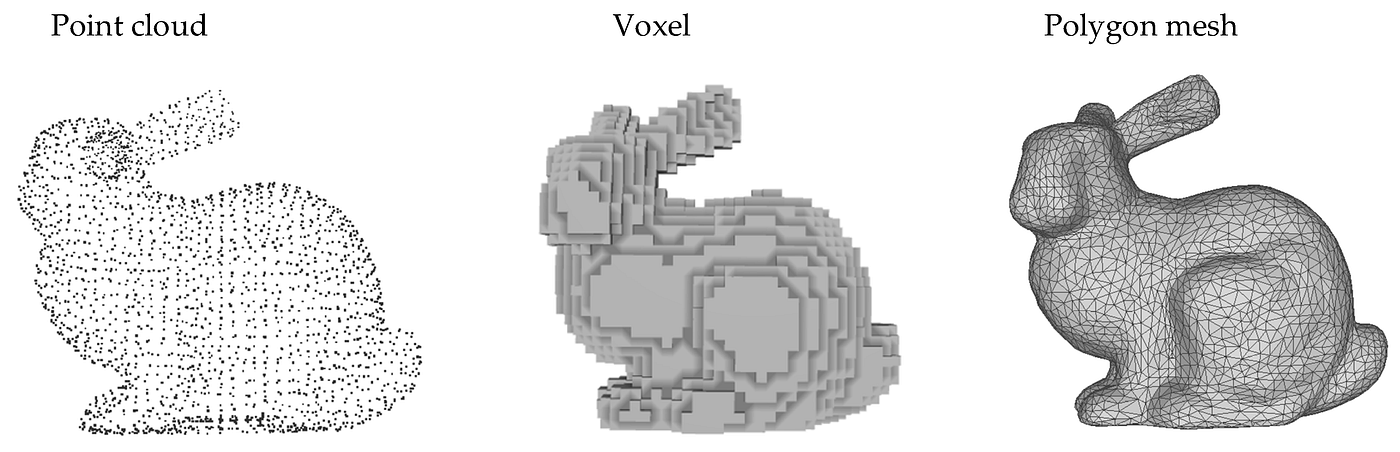
\includegraphics[width=0.9\textwidth]{figs/voxels.png}
    \caption{Different methods of representing 3D objects created by CT scans. \textbf{(i)}: Point Cloud Representation. \textbf{(ii)}: Voxel Representation. \textbf{(iii)}: Surface Mesh. (\cite{3DRepresentations})}
    \label{fig:3d_reps}
\end{figure}
\paragraph{Marching Cubes:} To take our voxels and turn them into a surface mesh we implement an algorithm called {\bf marching cubes} (\cite{MarchingCubes}):
\begin{enumerate}
    \item The stack of CT slices are converted to a \textbf{point cloud} representation. 
    \item A threshold value is set from which to cull elements of the tensor. If the value is less than the threshold, the element is set to 0.0, otherwise it is set to 1.0. The point cloud is now a binary representation of the tensor. The threshold value is selected such that only points remaining represent bones. 
    \item The algorithm selects \textbf{eight} adjacent elements of the tensor. These form a  ``cube'' in 3D space, where each point is a corner of the cube. There are 256 possible cubes; however, by exploiting their symmetry they can be reduced to 15 different unique cubes. 
    \item The cube is compared against a dictionary (Figure~\ref{fig:marching_cubes}) of the 15 cubes, which returns a predetermined set of polygons that best describe the surface created by those points (\cite{MarchingCubes}). 
    \item This is repeated for every \textbf{cube} in the tensor as the algorithm \textbf{marches} along all the elements in the tensor.
\end{enumerate}
\begin{figure}[H]
    \centering
    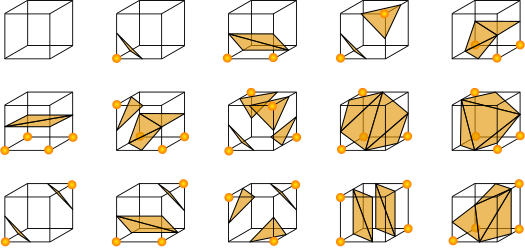
\includegraphics[width=0.8\textwidth]{figs/marching_cubes.png}
    \caption{The dictionary that maps the fifteen unique cubes to their corresponding surface meshes (\cite{MarchingCubes}).}
    \label{fig:marching_cubes}
\end{figure}

\paragraph{Shaders:} To speed up rendering, game and graphics engines use ``shaders''. These provide an interface for the engines to run rendering processes in parallel on a Graphics Processing Unit (GPU). Unity provides an API called ``Compute Shaders" which allows the user to define a function, that is not necessarily used for rendering, to run in parallel on the GPU, and pass information to and from the CPU by buffers.\\

Our implementation of the Marching Cubes algorithm works as described above. We choose our culling threshold so only bones are rendered (usually $\approx 0.85$). Additionally, we run the algorithm on the GPU in parallel with shaders (inspired by \cite{SebLague}) -- where the mesh for each cube is calculated concurrently by each GPU thread. Code for this is included in Appendix~\ref{sec:MarchingCubes} and the associated GitHub repository.

\subsubsection{Coordinate Transform using Horn's Method}
\label{coord:Coordinate Transform using Horn's Method}
To project the patient's anatomy onto their body, we must apply a coordinate transform to the rendered volume of the spine obtained from the marching cubes algorithm.\\

The first step is to find the Cartesian coordinates of the fiducial markers in the CT scans. We denote this set of points by the vector $x_c$ (CT Fiducials).\\

Since the fiducial markers are made of metal and are lying on top of the patient, they will appear as bright dots on the outer surface of the CT scan (as shown in Figure \ref{fig:mannequin}). While scrolling through the CT slices, the physician can click on these bright dots by aiming the controller at them one at a time. This will register their Cartesian coordinates in the CT frame of reference.\\

\begin{figure}[H]
    \centering
    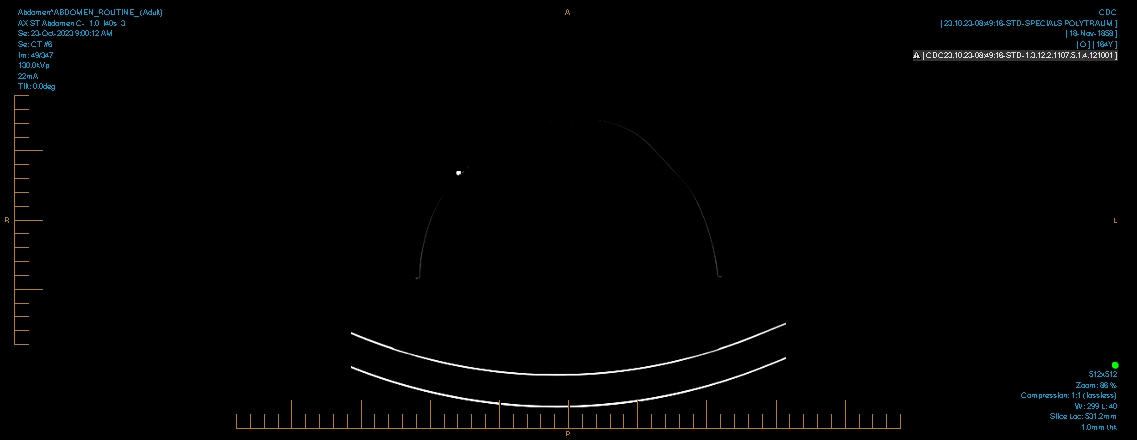
\includegraphics[width=0.8\textwidth]{figs/mannequin.jpg}
    \caption{A 2D CT slice of a hollow mannequin with a metal fiducial marker on its surface.}
    \label{fig:mannequin}
\end{figure}

To obtain the coordinates of the physical fiducial markers on the patient's body the physician can register them as spatial anchors as outlined in Section \ref{spa:Spatial Anchors}. We denote this set of points by the vector $x_p$ (Physical Fiducials).\\

With these two sets of coordinates, we can apply Horn's Algorithm. This mapping algorithm was recommended to us Dr. Robert Rohling, an expert in medical information systems at UBC. It is used to estimate "the translational (\textbf{t}), rotational (\textbf{R}), and uniform scalar (\textbf{s}) correspondence between two different Cartesian coordinate systems given a set of corresponding point pairs" (Robotics \cite{RoboticsRegistration}). In our case, the point pairs are the registered points in $x_p$ and $x_c$.

\begin{equation*}
    x_p = sRx_c + t
\end{equation*}

The goal of Horn's algorithm is to minimize the error (\(e_i\)) between corresponding fiducials when the transformation is applied to the CT fiducials ($x_c$).\\

We applied the following steps to find the best possible transformation between both coordinate frames.

\paragraph{Steps:}
\begin{enumerate}
    \item Find the centroid of each coordinate system where each fiducial has equal weighting. 
    \begin{align*}
        \overline{x}  = \frac{1}{N} \sum_i x_i 
    \end{align*}
    \item Create new coordinate systems \(x^{\prime}\) that are shifted by the centroids.
    \begin{align*}
        x^{\prime}_i = x_i - \overline{x}_i 
    \end{align*}
    \item Find the scale, by the ratio of the norm squared of each shifted coordinate system. 
    \begin{align*}
        s = \sqrt{\left( \sum_{i} \vert x^{\prime}_{p,i} \vert ^{2}  \right) \bigg/ \left( \sum_{i} \vert x^{\prime}_{c,i} \vert ^{2}  \right)} 
    \end{align*}
    \item Finally we find the rotation matrix, by minimizing the resulting error function - \(F(\theta ,\phi, \psi)\).
    \begin{align*}
        R = \text{argmin} \,2 \left( \sqrt{\left( \sum_{i} \vert x^{\prime}_{p,i} \vert ^{2}  \right) \left( \sum_{i} \vert x^{\prime}_{c,i} \vert ^{2}  \right)}  - \sum_{i}  x^{\prime}_{p,i} \cdot \left( R x^{\prime}_{c,i} \right) \right) 
    \end{align*}
    \item After which the translation ($t$) vector can be found:
    \begin{align*}
        t = \bar{x_p} - s R \bar{x}_c
    \end{align*}
\end{enumerate}

To find the rotation matrix \textbf{R}, we must perform an optimization function that minimizes the error between the Physical Fiducials and the transformed CT Fiducials. This is simple to do in Python; we can leverage the programming language's libraries such as SciPy.optimize.minimize. However, since Horn's Algorithm must be performed in real-time in the headset, it must be coded in C\#, with the .NET standard library.

The .NET standard library does not provide a package for scientific analysis. While there are .NET packages that do provide ways of optimizing functions, they have proven hard to include in our Unity projects because many do not target Android. 
Accordingly, we implemented our own optimizer \(Q\{E(\theta, \phi, \psi)\} \to (\theta, \phi, \psi)\). Our algorithm uses a {\bf prune and search} method to iteratively select candidate spaces. This drastically reduces the time complexity in searching for the 
minimizing rotation matrix. From a search space of about $\mathcal{O}(10^9)$ to about $\mathcal{O}(10^5)$. A software diagram of our algorithm is included in Figure~\ref{fig:optimizer} and a detailed description attached in Appendix~\ref{sec:Optimizer}. 
\begin{figure}[H]
    \centering
    
\includegraphics[width=0.9\textwidth]{"./figs/optimizer.pdf"}
    \caption{Flowchart of rotation optimizer.}
    \label{fig:optimizer}
\end{figure}

\subsection{Tests and Results}
Our main goal was to design and build an augmented reality system that has high precision and accuracy while maintaining ease of use for the user. We aimed to minimize the error between the intended needle trajectory and the actual needle trajectory. Since our system comprises numerous registrations and transformations, each with some associated error, we aimed to minimize the error of each of these components as much as possible so that the resultant propagated error was also minimized. Throughout the design of our system, we tried to quantify the error associated with our various registrations and transformations and quantify how these errors would affect the final system.

\subsubsection{Proposed Controller Attachment Tests}
The crucial thing to test with respect to the controller attachment is the accuracy of the calibration offset. To test the repeatability of the calibration procedure, we can perform the calibration multiple times and examine the variance of our results.\\

To test the accuracy of the calibration offset, we will add a marker to a piece of paper on a flat surface. A user will then put on the headset and draw a dot on the paper where they see the offset point in AR. By measuring the distance between the drawn dot and the marker, we get a measure of the accuracy of the calibration offset (Figure \ref{fig:controller_pointer_testing}).

\begin{figure}[H]
    \centering
    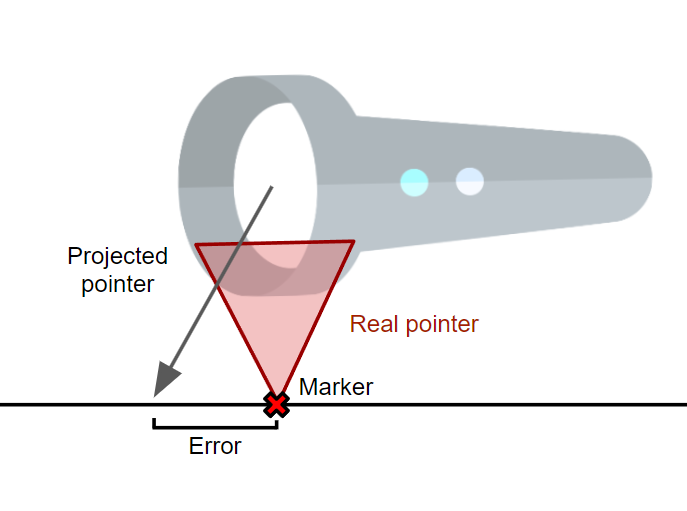
\includegraphics[width=0.6\textwidth]{figs/controller_pointer_testing.png}
    \caption{Testing controller calibration offset accuracy}
    \label{fig:controller_pointer_testing}
\end{figure}


\subsubsection{Horn's Algorithm Error Propagation}
To test how errors propagate we used a series of Monte Carlo simulations rather than finding an analytic solution. By altering different parameters of the simulation we found how they affect the error propagation in the system. A full Jupyter notebook can be found in Appendix 1. 
\paragraph{Methodology} The steps we took to conduct the simulations were as follows:
\begin{enumerate}
    \item Generate $N$ fiducicials. Each of these is situated in the XY plane, at some radius $R$ away from the origin. They are evenly spaced around the origin $\frac{2 \pi}{N}$ radians apart from each other.
    \item Each fiducial is randomly (normal distribution $\Delta \sim \text{Norm}(0, R / 5)$ perturbed in the X, Y and Z directions by some value. This step and the previous step simulate the curves and non uniform shape of the back of a patient. These points define the ``Registered Fiducials'' ($x_l$)
    \item A random transform is created, with scale (s), euler rotation (R) and translation (t). Then the same transform is applied to each of the fiducials.
    \item Each of the fiducials is perturbed once again by some small amount in $X_e$, $Y_e$ and $Z_e$ (each of them normally distributed: $\Delta_e \sim N(r, \sigma_e)$. We define a new random variable : 
    \[E_T = \sum_i^N \sqrt{X_{ei}^2 + Y_{ei}^2 + Z_{ei}^2}\]
    Where $i$ denotes the $i$th fiducial. This step simulates some random mean squared error (RMSE) that is added during the registration process. This new set of fiducials defines the ``CT Fiducials'' $x_r$.
    \item We run Horns Algorithm to map the CT Fidcucials to the Registered Fiducials ($\textbf{H} x_r \to x_{rt} \approx x_l$).
    \item We find the RMSE error between the Transformed CT Fiducials and the Registered Fiducials:
    \[
    E_R = \sum_i^N \sqrt{(X_{rt} - X_l)^2 + (Y_{rt} - Y_l)^2 + (Y_{rt} - Y_l)^2}
    \]
    \item To find how the errors propagate we compared the standard deviations and means of $E_T$ and $E_R$ (assuming they are normal distribution  by law of large numbers):
    \begin{align*}
        &E_T \sim \text{Norm}(\bar{T}, \sigma_T) \\
        &E_R \sim \text{Norm}(\bar{R}, \sigma_R)
    \end{align*}
    An example result of the simulation can be seen in Figure~\ref{fig:normal-dist}
    \begin{figure}[H]
        \centering
        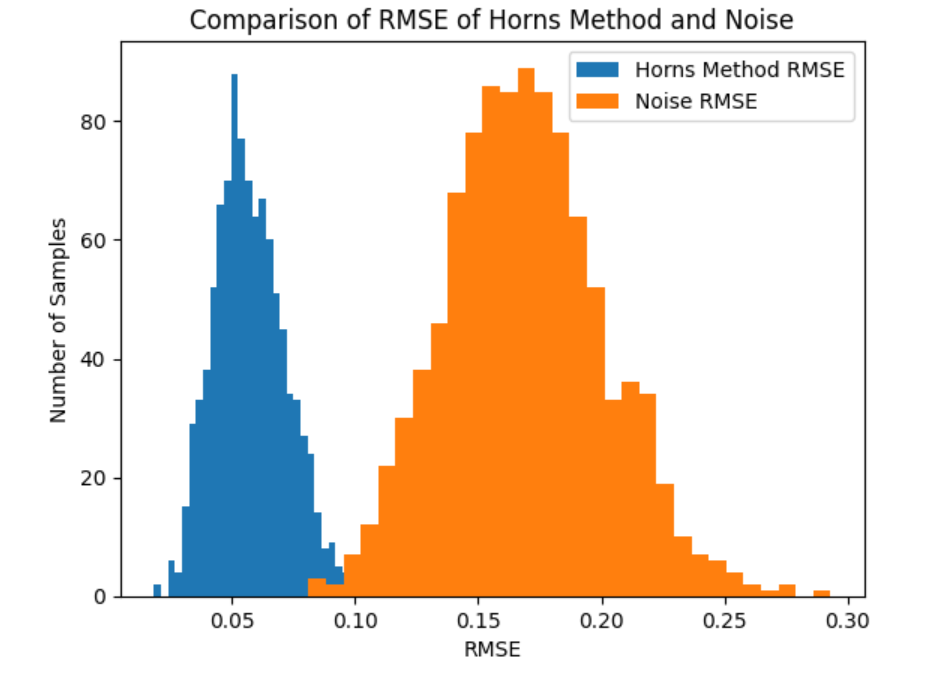
\includegraphics[width=0.8\textwidth]{figs/normal_dist.png}
        \caption{An example output from the simulation, comparing the input error and the error after Horn's Algorithm has been used to transform the noisy data.}
        \label{fig:normal-dist}
    \end{figure}
\end{enumerate}
\paragraph{Results} The results can be split into two parts:
\begin{enumerate}
    \item Error changes with respect to fiducial distance from orgin ($r$):
    \begin{align*}
    f_X(r) &= \frac{\text{X of } E_T (r)}{\text{X of } E_R (r)} \\
    \log|f_{\text{Mean}}(r)| &=  -0.438 \cdot r - 2.02 \quad \text{(Figure~\ref{fig:mean_error})}\\
    \log|f_{\text{STD}}(r)| &= -0.431 \cdot r - 3.2 \quad \text{(Figure~\ref{fig:std_error})}
    \end{align*}
    This is an exponential decay. Where initial increases in the distance from the origin decrease the errors in the registration greatly. However, this effect drops off as the distance becomes large. 
    \begin{figure}[H]
\centering
\begin{subfigure}{0.4\textwidth}
    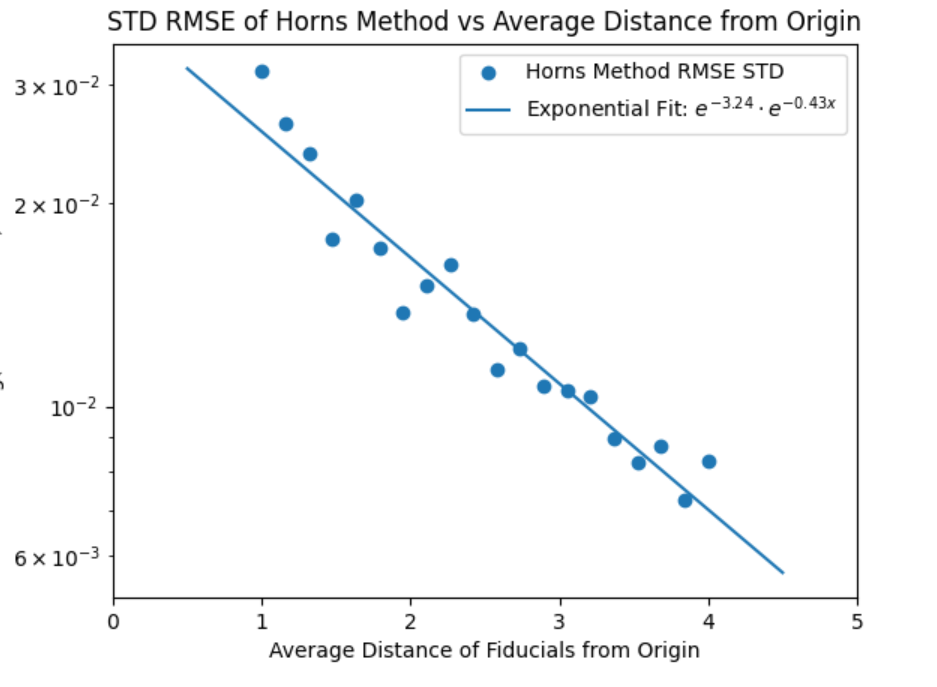
\includegraphics[width=\textwidth]{figs/horns_std.png}
    \caption{Shows how the standard deviation of errors changes as $r$ increases.}
    \label{fig:std_error}
\end{subfigure}
\hfill
\begin{subfigure}{0.4\textwidth}
    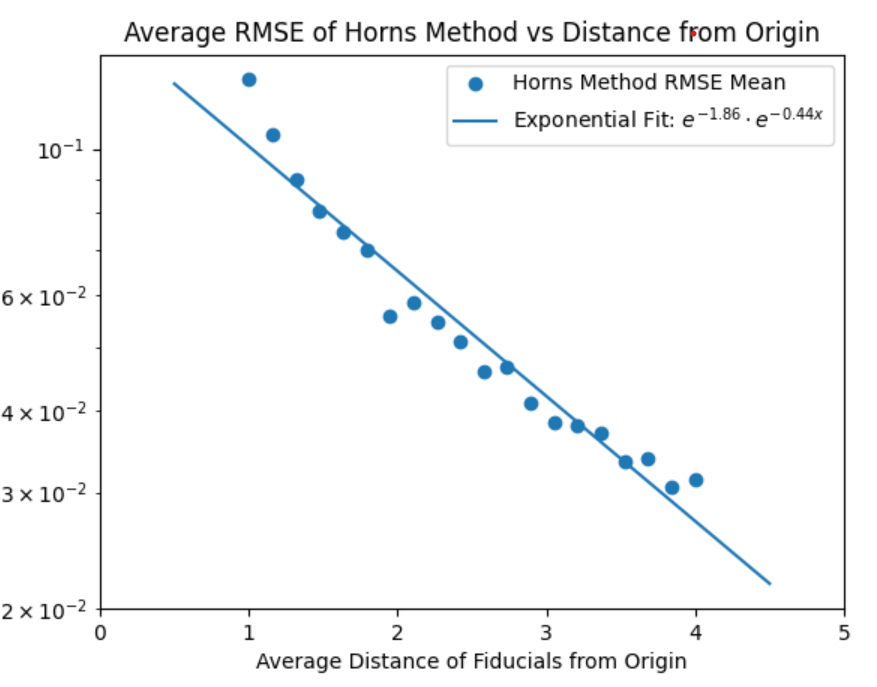
\includegraphics[width=\textwidth]{figs/horns.png}
    \caption{Shows how the mean of errors changes as $r$ increases.}
    \label{fig:mean_error}
\end{subfigure}        
\caption{The results of how the errors propagate from horns algorithm. Note these are logy graphs.}
\label{fig:error_propagation}
\end{figure}

\item Error changes with respect to the number of fiducials (N) - our results are only qualitative. However, the mean change in error increases with the N, while the STD (precision) decreases with N (Figure~\ref{fig:N_horns}). 
\begin{figure}[H]
\centering
\begin{subfigure}{0.4\textwidth}
    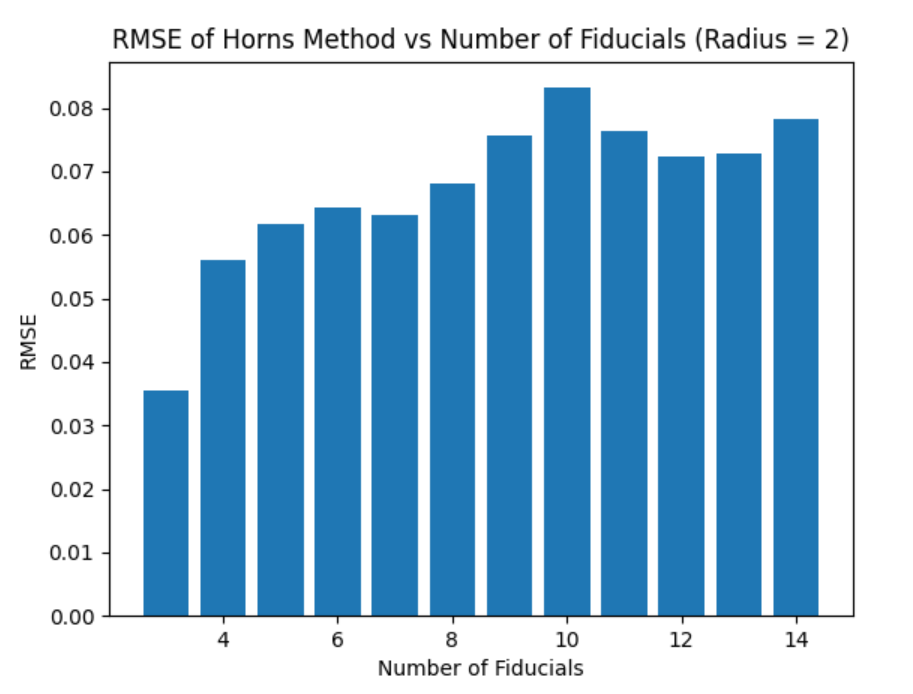
\includegraphics[width=\textwidth]{figs/horns_N.png}
    \caption{Shows how the mean of errors changes as $N$ increases.}
    \label{fig:N_mean}
\end{subfigure}
\hfill
\begin{subfigure}{0.4\textwidth}
    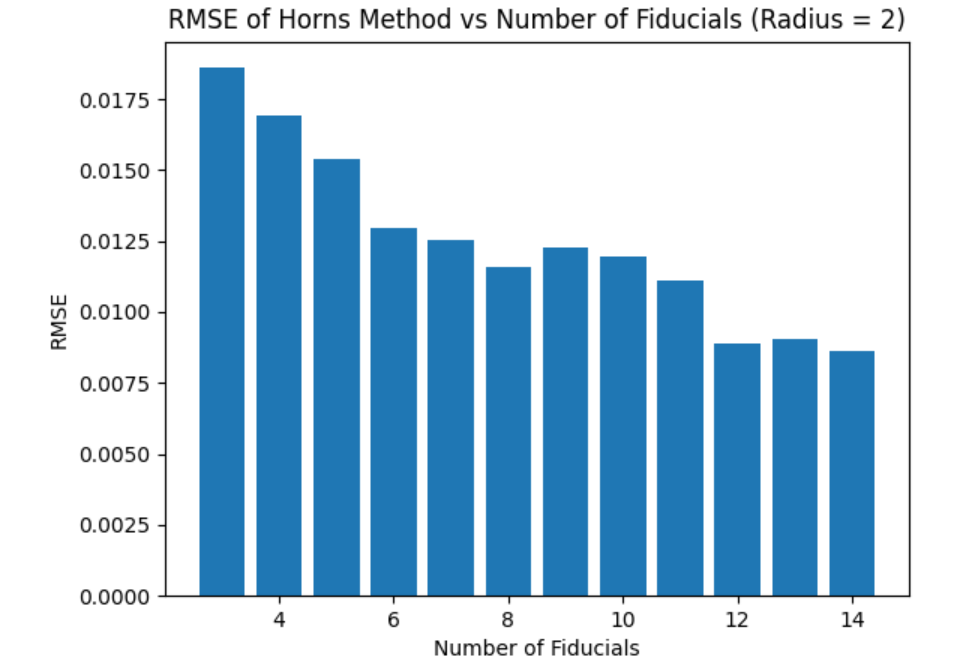
\includegraphics[width=\textwidth]{figs/horns_N_RMSE.png}
    \caption{Shows how the \textbf{standard deviation} of errors changes as $N$ increases.}
    \label{fig:N_std}
\end{subfigure}        
\caption{The results of how the errors propagate from horns algorithm. Note these are logy graphs.}
\label{fig:N_horns}
\end{figure}
\end{enumerate}
\paragraph{Key Takeaways and Limitations.} This analysis suggests that we should have a large distance between the fiducials and keep the number of fiducials between three and five. However, this analysis only shows the average error between coordinate systems and does not show localised errors. It will be important to investigate localised errors further as they are more relevant to our application.\\

So far, we have only used Horn's algorithm on simulations using sets of generated sample points with random error. We are assuming that the real system will behave similarly to this simulation, but this may be a false assumption. This limits the conclusions we can make from these simulations. We will need to apply this algorithm to the actual coordinates of fiducial markers registered using our spatial anchoring procedure and see if we obtain acceptable results.
\section{Conclusions}
\subsection{Controller Attachments}
We have 3D printed controller attachment prototypes and qualitatively tested the rigidity of their connection to the Quest 3 controllers (Figure \ref{fig:controller_pointer_picture}). In addition, we have developed a software implementation of the proper calibration procedure up until the optimization function.

\begin{figure}[H]
    \centering
    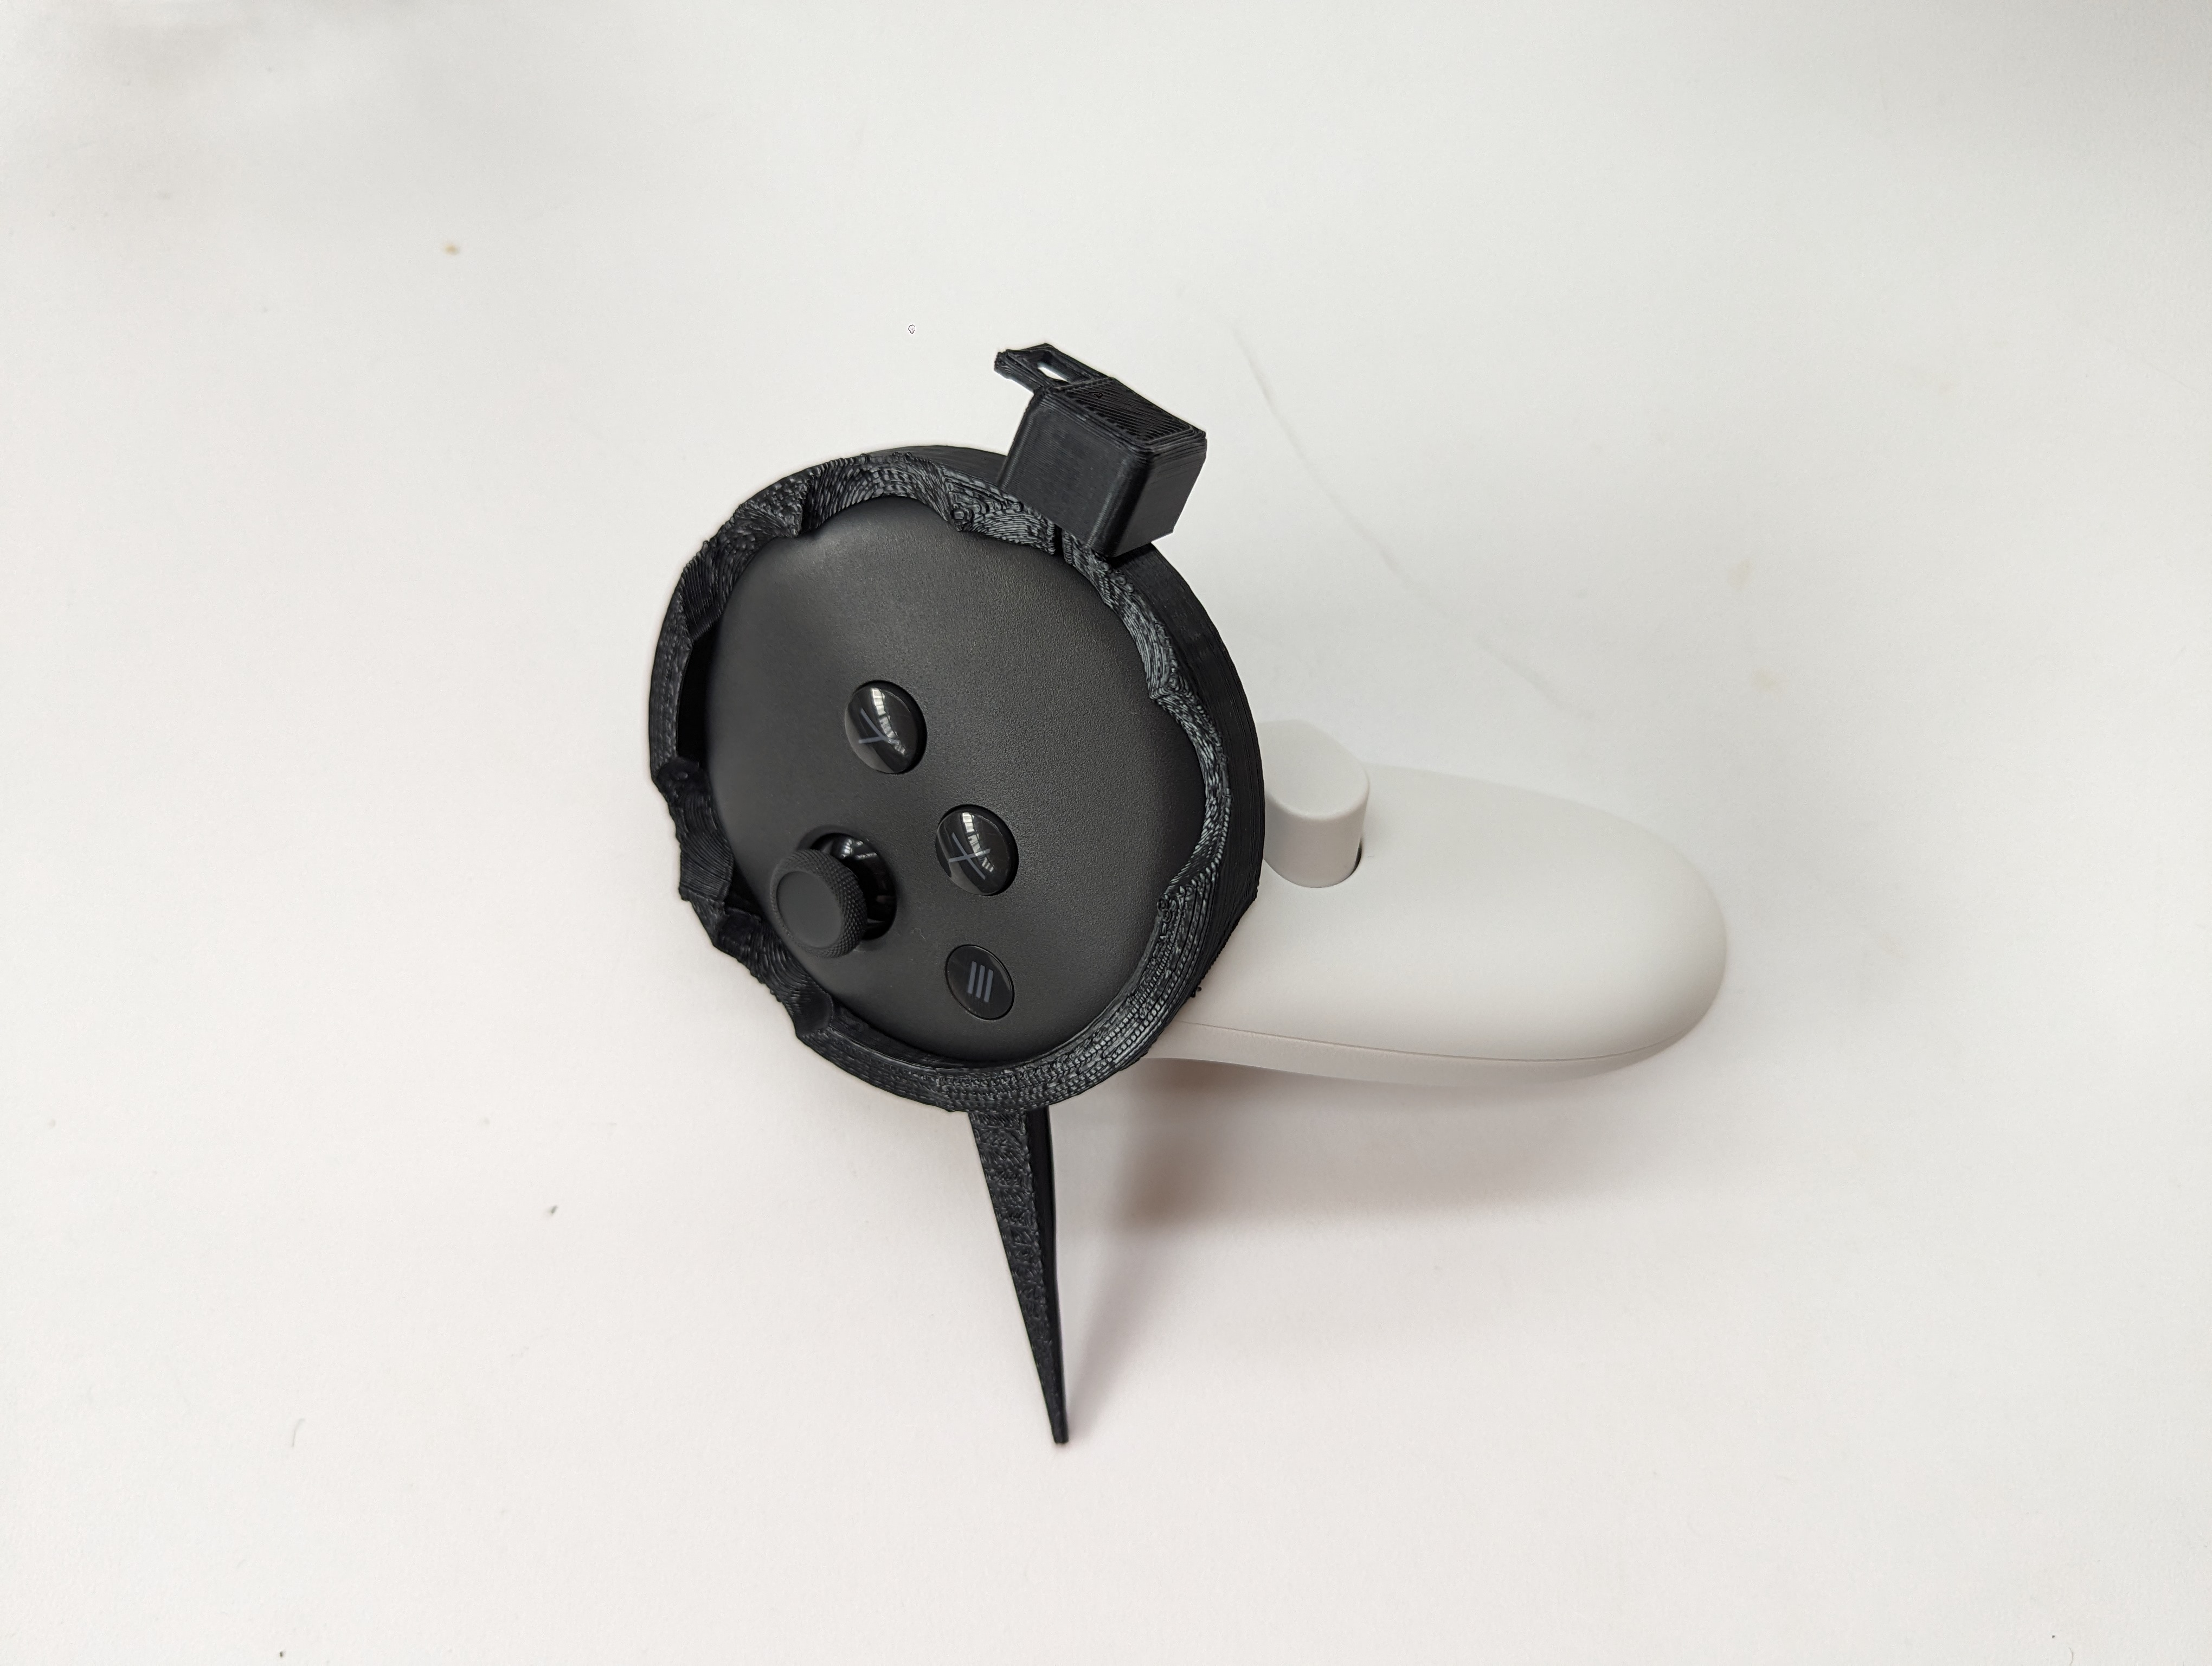
\includegraphics[width=0.3\textwidth]{figs/quest_controller.jpg}
    \caption{Controller pointer attachment prototype}
    \label{fig:controller_pointer_picture}
\end{figure}


\subsection{Spatial Anchors}
We have created a Unity demo to allow the user to place and remove spatial anchors at an arbitrary location with respect to the controller.
\subsection{Horn's Algorithm}
We have finished writing an implementation of the Horn's algorithm in a Jupyter notebook and C\# script. The aforementioned error propagation simulations for Horn's algorithm has given us insight into the effects of uncertainty on the mapping.
\subsection{3D Meshing}
We have fully implemented volumetric 3D rendering in Unity (Figure \ref{fig:volumetric_rendering}). The rendering is interactable and transformable, allowing for us to define its location with spatial anchors in the future.

\begin{figure}[H]
    \centering
    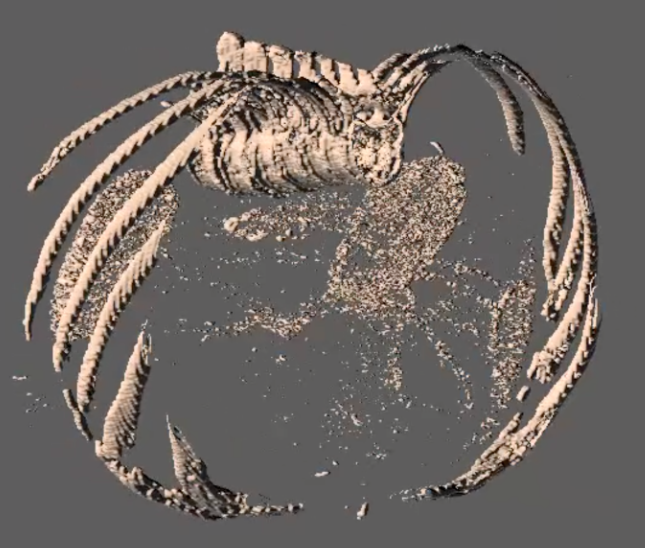
\includegraphics[width=0.3\textwidth]{figs/volumetric_rendering.png}
    \caption{Volumetric rendering of CT scans rendered in Unity}
    \label{fig:volumetric_rendering}
\end{figure}


\section{Recommendations}
This is a two year project and we plan to implement all the features outlined in our Proposed Solution (Section~\ref{sec:ProposedSolution}). While we have some of the missing features are written out in either Python or C\# we still need to integrate them. The progress of incomplete sub-systems is written out below:
\begin{enumerate}
    \item Registration with Horn's Algorithm -- Horns algorithm written out in C\# but not integrated with a Unity game world (``scene"). Registration with spatial anchors is complete but not integrated with our demo.
    \item Slice Selection -- Selection is implemented and integrated with our demo. However, we are missing the ability to situate the slices in the scene (see above) and draw a desired directory on the slices. 
    \item Controller Registration -- Mathematical theory has been worked out but not implemented in code.
    \item Controller Tracking and Angle Feedback -- Not implemented on any platform.
    \item Runtime downloading of DICOM files from hospital servers, and conversion and extraction of CT Slices -- Not implemented on any platform.
\end{enumerate}
Additionally, we need to evaluate the effectiveness of AR as a means of guidance in clinical settings. This includes evaluating the:
\begin{enumerate}
    \item Tracking accuracy of the Meta Quest 3 controllers.
    \item Consistency of Quest 3 headset in situating itself over long periods of time.
    \item User accuracy using our technique. We recommend doing this by conducting tests where the headset user is asked to insert a needle into a foam block using only the visual guidance of the headset. The insertion and end points of the needle through the foam block would then be compared with the intended trajectory to evaluate the accuracy of the system.
    \item Effectiveness of the different sub-systems our technique uses in assisting the user (e.g. does the 3D model provide better assistance to the user than hand tracking).
    \item User experience of our systems based on feedback from clinicians. 
\end{enumerate}
\section{Deliverables}
\subsection{Mechanical}
CAD models for the controller attachments and testing rigs can be found in an \href{https://cad.onshape.com/documents/a7669772db1e8cf42f0d84d7/w/a372f52852661928ae6b39d4/e/6cbc84bf2eabff7db7f6d995?renderMode=0&uiState=661c9dc0dc1f8708bbbcbccf}{Onshape document.}
\subsection{Software}
A majority of our work is contained in \href{https://github.com/okim1227/AR-Spinal-Injection.git}{\underline{a GitHub Repository}} including working Unity scenes, Jupyter (Python) Notebooks and C\# scripts.
\begin{enumerate}
    \item ``\textbf{ProjectFair/}'' is a Unity scene which implements:
      \begin{enumerate}[label=\alph*.]
    \item Slice Selection,
    \item 3D Modelling with Marching Cubes.
  \end{enumerate}
  \item ``\textbf{Notebooks/Horns.ipynb}'' -- Python Jupyter Notebook showing how we implement Horn's Algorithm and it's error propagation (.html file included as well). 
  \item ``\textbf{Scripts/Horns.cs}'' -- Unity C\# file that uses Horns Algorithm and implements our rotation function optimiser.
\end{enumerate}
\section{References}
\printbibliography
\end{document}
